\documentclass[conference]{IEEEtran}
\IEEEoverridecommandlockouts

\usepackage{cite}
\usepackage{amsmath,amssymb}
\usepackage{graphicx}
\usepackage{booktabs}
\usepackage{textcomp}
\usepackage{xcolor}
\usepackage{hyperref}

\graphicspath{{images/}}

\begin{document}

\title{How World-Model Quality Shapes Model-Based Control: Imagination Horizon, Data Size and a Pixel-Based CartPole/Pong Study}

\author{
\begin{tabular}{ccc}
\begin{tabular}{c}
\textbf{Jithin Shaji}\\
Department of CSE\\
IIIT Kottayam\\
Kerala, India\\
jithin23bcs14@iiitkottayam.ac.in\\
2023BCS0014
\end{tabular}
&
\begin{tabular}{c}
\textbf{J Glen Enosh}\\
Department of CSE\\
IIIT Kottayam\\
Kerala, India\\
glen23bcd61@iiitkottayam.ac.in\\
2023BCD0061
\end{tabular}
&
\begin{tabular}{c}
\textbf{Aysha Lintha}\\
Department of CSE\\
IIIT Kottayam\\
Kerala, India\\
aysha23bcs183@iiitkottayam.ac.in\\
2023BCS0183
\end{tabular}
\end{tabular}
}

\maketitle

\begin{abstract}
We study how the quality of a learned world model affects model-based control, with a focus on the imagination horizon. Our approach uses a convolutional VAE, a probabilistic GRU for predicting the next latent state, reward and episode termination, and a random-shooting model-predictive controller (MPC) that plans through imagined trajectories. On pixel-based CartPole, trained on 20k transitions, latent prediction error grows with horizon and performs no better than a copy-last-latent baseline beyond roughly horizon of 10, yet planning with that horizon achieves a higher mean return than random actions and performs comparably to a DQN trained for 80,000 steps. A Horizon of 1 is worse than random. Model quality is unstable with 1,000 transitions, with two of three seeds collapsing, but stabilizes with 5,000 transitions. In a matched-data comparison the world-model planner shows no clear advantage over DQN given the same 20k environment steps, so we do not claim better sample efficiency. On Atari Pong a model with a foreground-weighted loss beats the copy baseline but control remains weak. Our findings overall show that the effectiveness of model-based control depends on both the fidelity of learned dynamics and the planning horizon, with the benefits of longer rollouts limited by accumulated prediction error.
\end{abstract}

\begin{IEEEkeywords}
world models, model-based reinforcement learning, variational autoencoder, recurrent dynamics, model-predictive control, imagination horizon
\end{IEEEkeywords}

%--------------------------------------------------------------------
\section{Introduction}
Model-based reinforcement learning (MBRL) uses learned environment dynamics to plan actions or generate imagined experience for policy learning. When observations are images, the model usually works in a learned latent space \cite{ha2018,hafner2019,hafner2020,hafner2023}. The practical question we ask here is not whether a world model can be trained, but how its quality, measured by prediction error, determines how useful it is for control, and how far into the future its imagined trajectories can be trusted.

We evaluate four hypotheses:
\begin{itemize}
    \item \textbf{H1:} Increasing training-data size improves
    world-model quality.

    \item \textbf{H2:} Prediction error increases with the
    imagination horizon.

    \item \textbf{H3:} Control performance peaks at an
    intermediate imagination horizon.

    \item \textbf{H4:} A learned world model enables control
    performance to exceed that of a random policy.
\end{itemize}
We evaluate on CartPole from pixels (main study) and on Atari Pong (extension), compared with a random policy and a model-free DQN \cite{mnih2015}.

\emph{Contributions:} (i) a compact, fully reproducible VAE + probabilistic GRU + random-shooting MPC pipeline; (ii) a controlled study of error versus horizon, data size and control return, including multi-seed runs; (iii) matched-data comparisons against DQN and extra studies of planning budget and task transfer; (iv) an honest account of where the approach fails, notably on Pong.

%--------------------------------------------------------------------
\section{Literature Review}
World Models \cite{ha2018} trains a VAE and a recurrent model, then a small controller on its latent representations. PlaNet \cite{hafner2019} introduced latent-space planning with a recurrent state-space model (RSSM), while Dreamer \cite{hafner2020,hafner2023} learns behaviours by backpropagating through imagined latent rollouts. SimPLe \cite{kaiser2020} and IRIS \cite{micheli2023} demonstrate the use of learned environment models for policy optimization in Atari environments.

A fundamental challenge in model-based reinforcement learning is the compounding of model prediction errors over imagined trajectories. MBPO \cite{janner2019} addresses this issue by restricting model-generated rollout lengths, motivating our investigation of how imagination horizon affects both predictive accuracy and control performance. Embed to Control \cite{watter2015} and probabilistic ensembles \cite{chua2018} use learned models for planning with random-shooting or sampling-based optimisation. Recent analysis of Atari Pong \cite{pong2026} reports that strong agents can contain weak world models in which the small ball disappears, and proposes an auxiliary reconstruction loss on the ball region. Building up from this observation, we use a foreground-weighted reconstruction loss and observe similar difficulties in predicting ball dynamics.

\begin{table}[t]
\caption{Positioning of this work}
\label{tab:positioning}
\centering
\begin{tabular}{@{}lll@{}}
\toprule
Method & Latent model & Use of model \\
\midrule
World Models \cite{ha2018} & VAE + MDN-RNN & Evolved controller \\
PlaNet \cite{hafner2019} & RSSM & Latent planning (CEM) \\
Dreamer \cite{hafner2020} & RSSM & Actor-critic in imagination \\
MBPO \cite{janner2019} & Ensemble (state) & Short rollouts for SAC \\
This work & VAE + GRU & Random-shooting MPC \\
\bottomrule
\end{tabular}
\end{table}

%--------------------------------------------------------------------
\section{Methodology}
\subsection{World model}
The observations made are $64\times64$ grayscale frames, with two consecutive frames stacked for CartPole and 4 for Pong to provide temporal information. A convolutional VAE \cite{kingma2013} maps these observations to a 32-dimensional latent representation. It is trained using a reconstruction loss and a $\beta$-weighted KL term ($\beta{=}0.03$ for CartPole). 

The latent dynamics  are modeled in a single-layer GRU \cite{cho2014} with 256 hidden units (512 for Pong). Given the latent $z_t$, action $a_t$ and hidden state $h_t$, the GRU outputs a diagonal Gaussian over the next latent state $z_{t+1}$, along with a reward prediction and a episode termination probability. This model is trained with Gaussian negative log-likelihood on sequences of length 16, so imagined rollouts can be sampled. The VAE and the dynamics model are trained separately. The VAE is frozen before the dynamics training, and the GRU receives the VAE posterior means.

\subsection{Planning}
We use random-shooting MPC. At each decision step, the controller samples 256 candidate action sequences of length $H$. The GRU hidden state is initialized by processing the most recent eight real latent-action pairs, after which each candidate sequence is evaluated through imagined rollouts. Candidate sequences are scored using predicted discounted rewards weighted by predicted survival probabilities. The controller executes the first action of the highest-scoring sequence and replans at the next step. Episodes are capped at 200 environment steps.

\subsection{Baselines and metrics}
We compare against a uniformly random policy and a convolutional neural network (CNN) DQN \cite{mnih2015} trained on the same stacked-frame representation. The primary DQN baseline is trained for 80k environment steps across three seeds. Additional comparisons use budgets of 20k and 40k steps.

World-model prediction quality is evaluated using latent mean squared error normalized by the variance of the test-set latent representations (NMSE). We compare this error against a persistence baseline that predicts $z_{t+1}=z_t$, and also report VAE reconstruction error and pixel-space MSE. Prediction errors are evaluated over 512 initial states, with standard errors reported where applicable.

For CartPole, the world-model training dataset combines transitions collected using random actions and a noisy balancing heuristic in equal proportions. This mixture provides longer trajectories than random interaction alone, but introduces a data-collection bias. We therefore conduct an additional experiment using random-policy data exclusively to assess its effect on model quality and control performance.

%--------------------------------------------------------------------
\section{Results and Discussions}
\subsection{World-model quality (CartPole, 20k transitions)}
The VAE achieves a reconstruction MSE of $4\times10^{-5}$, indicating that it can effectively reconstruct the input frames. The dynamics model also performs better than simply copying the previous latent state, achieving a one-step NMSE of $0.0029$ compared with $0.0109$ for the copy baseline. However, prediction errors increase as the imagination horizon grows, supporting H2. The model performs better than the baseline only for horizons shorter than $10$ steps, with comparable errors at $H=10$ ($0.23$ versus $0.24$). Beyond this point, the error increases considerably, reaching $1.55$ at $H=20$, compared with $0.73$ for the baseline. This trend is also observable in the imagined frames in Fig.~\ref{fig:film}: the predictions remain recognisable at $H=10$, become noticeably degraded at $H=20$, and largely dropdown at horizons of $30$–$40$ steps.

\begin{figure}[t]
\centering
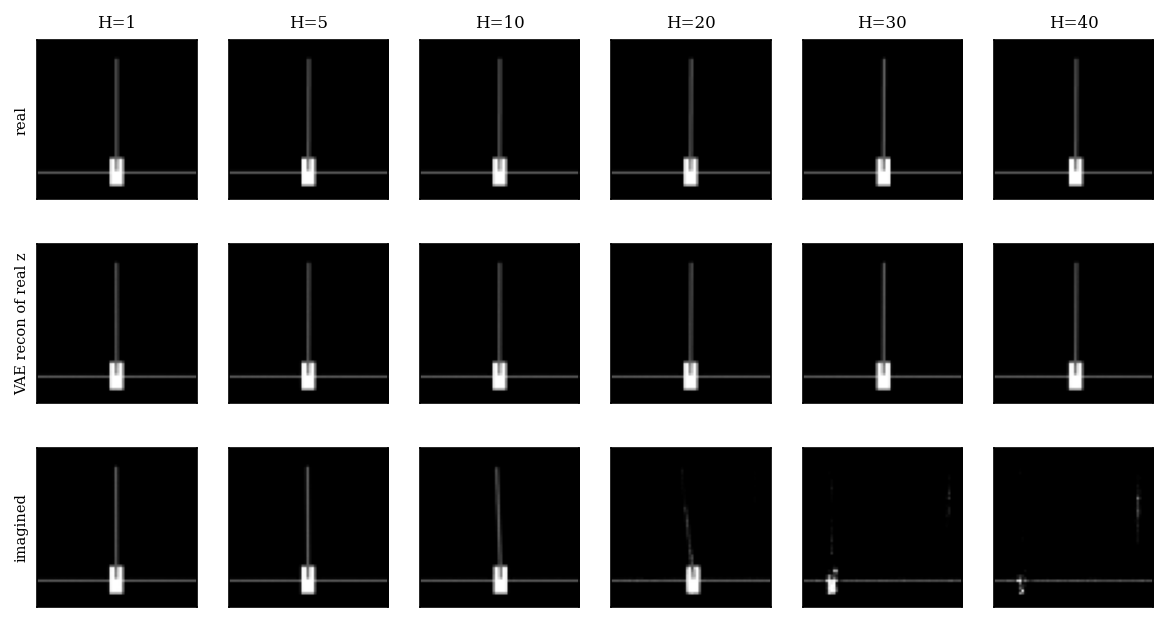
\includegraphics[width=\columnwidth]{f_film.png}
\caption{Real frames, VAE reconstructions of the real latent, and imagined frames at horizons 1 to 40 for CartPole.}
\label{fig:film}
\end{figure}

\begin{table}[t]
\caption{Latent NMSE versus horizon (20k transitions, sampled rollouts)}
\label{tab:nmse}
\centering
\begin{tabular}{@{}lcccccc@{}}
\toprule
$H$ & 1 & 5 & 10 & 20 & 30 & 40 \\
\midrule
Model & 0.006 & 0.064 & 0.23 & 1.55 & 5.80 & 17.5 \\
Copy $z_t$ & 0.004 & 0.074 & 0.24 & 0.73 & 1.19 & 1.45 \\
\bottomrule
\end{tabular}
\end{table}

\begin{figure}[t]
\centering
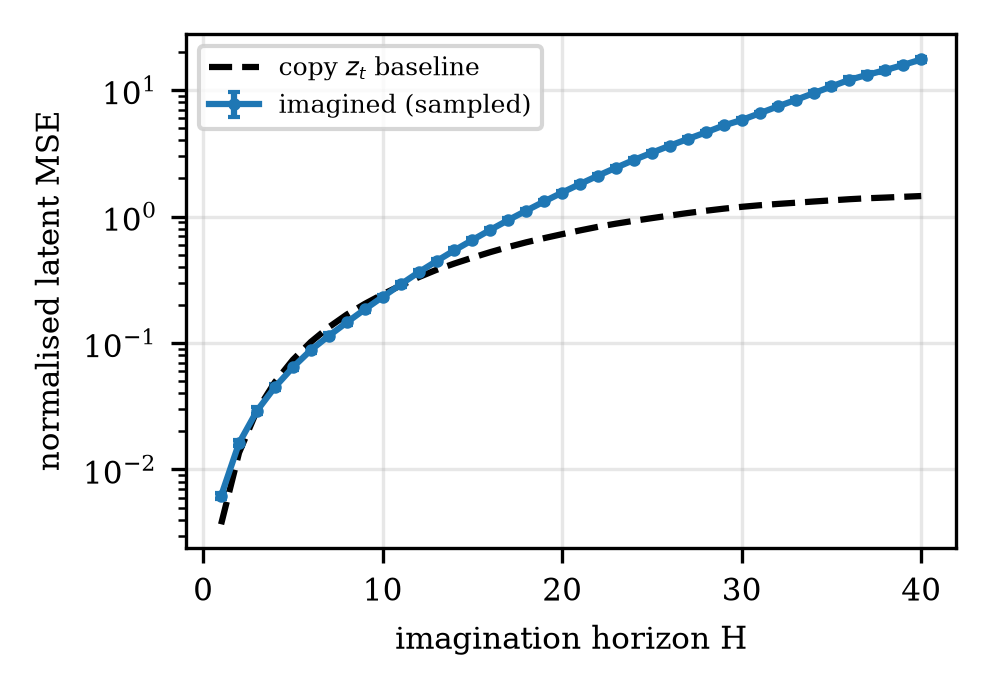
\includegraphics[width=\columnwidth]{f_error.png}
\caption{Latent NMSE of imagined rollouts versus horizon, with the copy-$z_t$ baseline (log scale).}
\label{fig:error}
\end{figure}

\subsection{Effect of training-set size (H1)}
With only $1K$ transitions, the model is unreliable, as 2 out of 3 seeds collapse, producing a VAE reconstruction MSE of $0.0147$ and nearly empty reconstructed images. The remaining seed performs reasonably well, with MPC returns ranging from $13.6$ to $22.0$. In contrast, all seeds remain stable with $5K$ or more transitions. Reconstruction MSE decreases from $1.4\times10^{-4}$ at $5{,}000$ transitions to $4\times10^{-5}$ at $20{,}000$, while the mean MPC return increases from $54.5$ to $68.7$ and $94.9$ for $5{,}000$, $10{,}000$, and $20{,}000$ transitions, respectively, as shown in Fig.~\ref{fig:data}. These results support H1, suggesting that sufficient training data is necessary for stable learning, with further improvements as the dataset grows. However, the one-step NMSE remains approximately constant at $0.003$ across the $5{,}000$–$20{,}000$ range, and the substantial variation across seeds at $10{,}000$ transitions, with returns ranging from $24.6$ to $136.2$, indicates that the observed performance trend is noisy.

\begin{figure}[t]
\centering
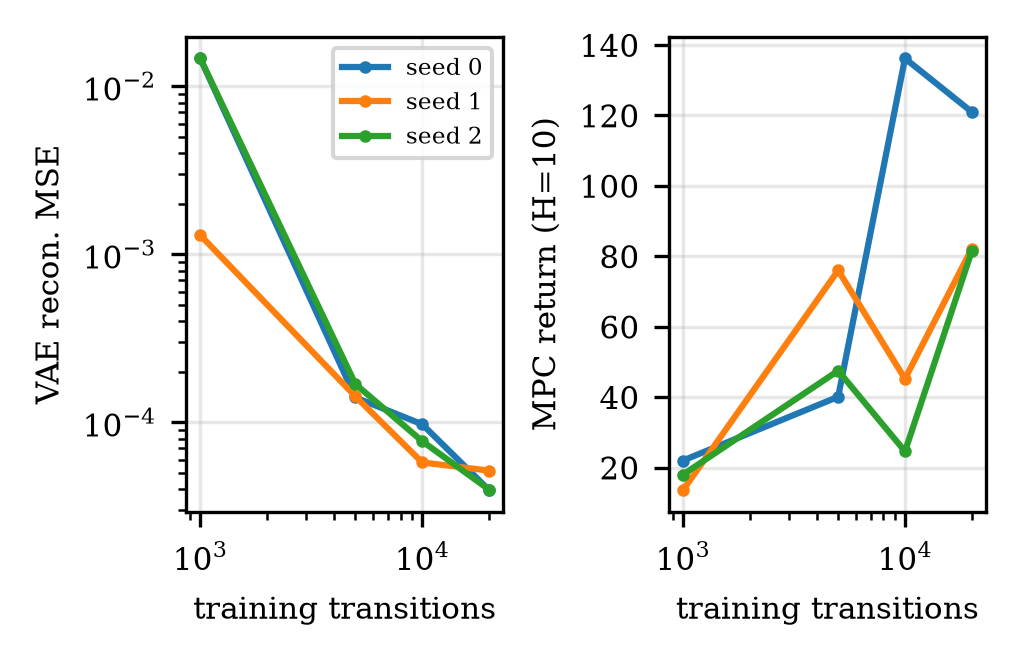
\includegraphics[width=\columnwidth]{f_data.png}
\caption{Left: VAE reconstruction MSE versus data size (3 seeds). Right: MPC return ($H{=}10$) versus data size.}
\label{fig:data}
\end{figure}

\subsection{Control versus imagination horizon (H3, H4)}
The mean returns over 20 episodes are reported in Fig.~\ref{fig:control} and Table~\ref{tab:cartpole}. The random policy achieves a return of $19.4$, while MPC obtains $10.4$, $39.9$, $118.6$, $106.7$, $92.2$, and $92.6$ for planning horizons of $H=1$, $H=5$, $H=10$, $H=20$, $H=30$, and $H=40$, respectively. DQN achieves returns of $103.8$, $77.6$, and $125.1$ across the 3 seeds, with a mean of $102.2$. The poor performance at $H=1$ can be correlated to the limited information available for planning when the reward is constant for surviving. Performance improves substantially as the horizon increases to $H=10$, followed by a gradual decline. This overall trend supports H3, with the best performance occurring around horizons of $10$–$20$ steps and a degradation at longer horizons as model predictions become less reliable. However, the difference between $H=10$ and $H=20$ is not statistically significant given their standard errors of approximately $8$–$9$. Similarly, the decline in return at $H=30$–$40$ is relatively small compared with the increase in model prediction error. This may be because MPC replans at every step, limiting its dependence on predictions far into the future. Finally, the results support H4 by demonstrating that planning with an imperfect model can still be effective: MPC with $H=10$ achieves performance comparable to a model-free agent trained for $80{,}000$ steps, despite using only $20{,}000$ collected transitions.

\begin{table}[t]
\caption{CartPole mean return (20 episodes, mean over seeds for DQN)}
\label{tab:cartpole}
\centering
\begin{tabular}{@{}lc@{}}
\toprule
Method & Return \\
\midrule
Random & 19.4 \\
MPC $H{=}1$ / 5 & 10.4 / 39.9 \\
MPC $H{=}10$ / 20 & 118.6 / 106.7 \\
MPC $H{=}30$ / 40 & 92.2 / 92.6 \\
DQN 80k steps (3 seeds) & 102.2 \\
\bottomrule
\end{tabular}
\end{table}

\begin{figure}[t]
\centering
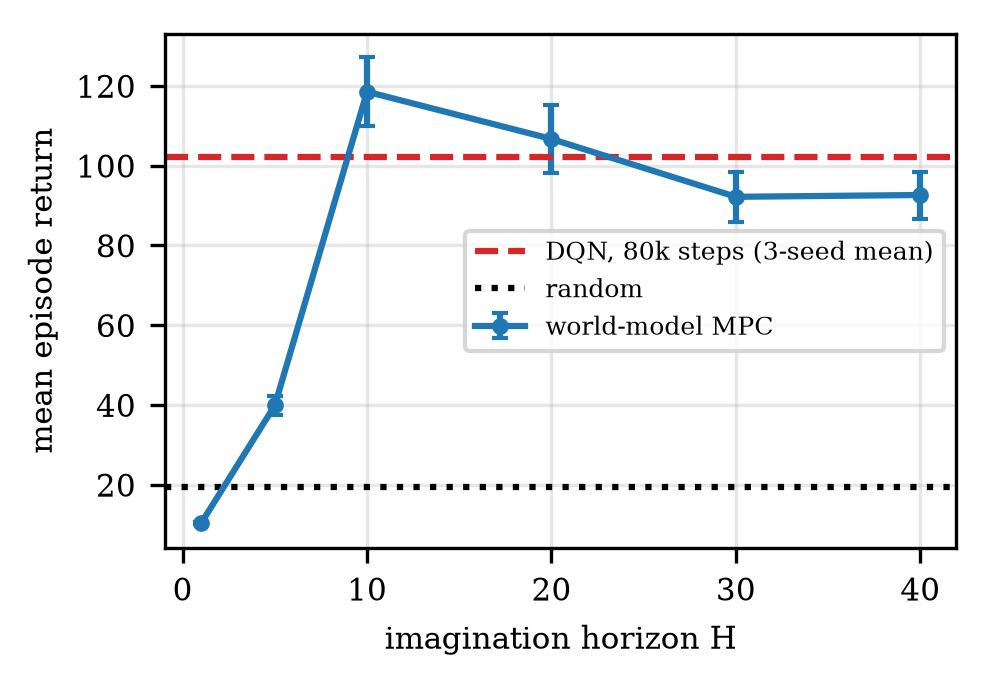
\includegraphics[width=\columnwidth]{f_control.png}
\caption{Planning return versus imagination horizon with random and DQN references.}
\label{fig:control}
\end{figure}

\subsection{Matched-data comparison with DQN}
To evaluate the sample efficiency of the world model, we compared MPC against DQN trained with 20k and 40k environment steps (Fig.~\ref{fig:matched}). MPC with $H{=}10$, trained using 20k transitions across 3 model seeds, achieves a mean return of 94.9, compared to $85.6\pm12.0$ for DQN-20k across 5 seeds. However, this difference is within the observed variation, while DQN-40k achieves a higher return of $116.3\pm16.0$. When trained only on randomly collected data, without the heuristic episodes, the world model performs considerably worse, with a reconstruction MSE of $3.7\times10^{-3}$ and NMSE exceeding the copy baseline at every horizon (14.1 vs.\ 1.3 at $H{=}20$). Consequently, MPC returns drop to 50.7, 68.8, and 71.1 for $H{=}5$, 10, and 20, respectively, falling below DQN-20k. Overall, our experiments do not support the claim that the world model learns more effectively from less data. Its performance also depends on the hand-written heuristic used during data collection.

\begin{figure}[t]
\centering
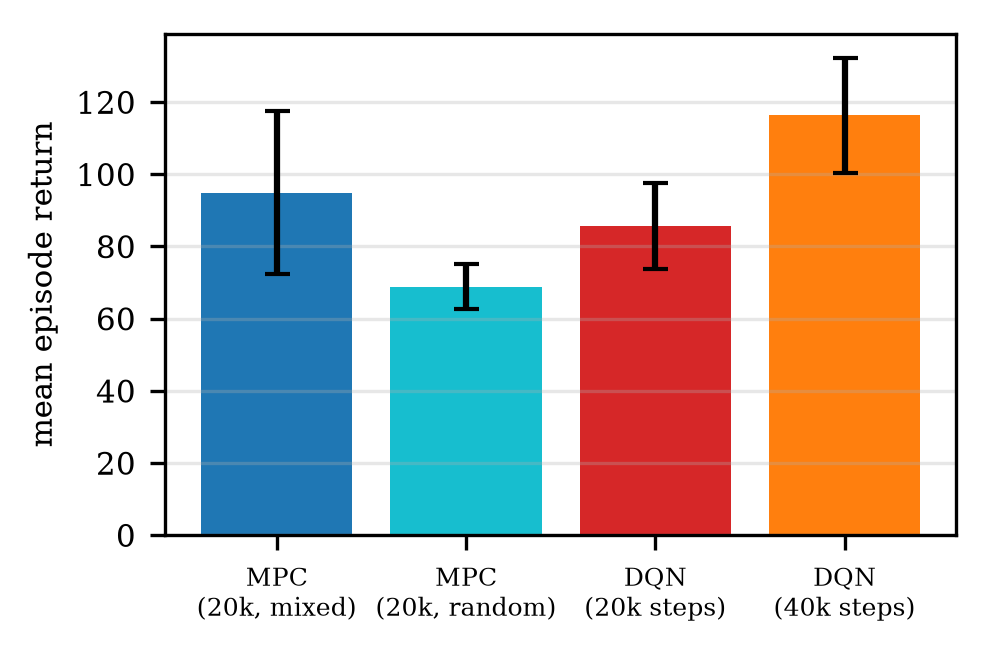
\includegraphics[width=\columnwidth]{f_matched.png}
\caption{Matched-data comparison (mean $\pm$ std over seeds).}
\label{fig:matched}
\end{figure}

\subsection{Planning budget and task transfer}
We also evaluated the effect of the number of candidate sequences on MPC performance for $H{=}10$ across 3 seeds. Mean returns are 94.7, 103.4, 107.2, 105.3, and 102.8 for 16, 64, 256, 1024, and 4096 candidates, respectively. Performance largely saturates between 64 and 256 candidates, suggesting that increasing the search space further does not improve returns. To evaluate whether the learned world model can be reused for new tasks, we retrained only the reward head using relabelled stored transitions. For the `upright' task, with reward $1-|\theta|/0.2095$, MPC achieves returns of 101.6 at $H{=}10$ and 106.5 at $H{=}20$, compared to 12.1 for the random policy. Using the stale reward head yields 83.8 and 68.9, respectively. However, DQN trained from scratch achieves 102.6 with 20k steps and 92.3 with 40k steps (2 seeds), indicating that reward-head adaptation performs comparably to DQN rather than outperforming it. Transfer is less successful on the `left' task, where the reward depends on whether the cart is left of centre. MPC obtains returns of 18.9 and 26.7, compared to 8.1 for the random policy, while DQN achieves 38.2 and 52.3 with 20k and 40k steps, respectively. We did not investigate the cause of this failure. One possible explanation, which remains untested, is that the latent representation captures cart position too coarsely to model the sharp threshold in the reward function.

\subsection{Atari Pong (extension)}
Our initial Pong experiment failed because the ball was lost during frame preprocessing and VAE reconstruction. We addressed this using cropping, background subtraction, a foreground-weighted reconstruction loss with a weight of 50, and 30k transitions collected by mixing a tracking policy with random actions. Following these changes, the VAE achieves a reconstruction MSE of $3.6\times10^{-4}$, and the learned dynamics model outperforms the copy baseline at every prediction horizon, with NMSE values of 0.17 vs.\ 0.33 at $H{=}1$ and 1.02 vs.\ 2.06 at $H{=}20$. However, imagined ball positions remain unreliable, with drifting and missing balls observed in the generated filmstrips. Control performance is also limited (Table~\ref{tab:pong}). Mean returns improve with increasing horizon, reaching $-19.9$, $-19.8$, $-15.8$, and $-12.7$, compared to $-20.6$ for the random policy, but MPC never wins a game, with the best single-episode return being $-4$. In comparison, a DQN trained for 300k steps achieves a return of $+11$. However, its deterministic evaluation produces identical results across all 20 episodes, effectively representing a single trajectory rather than 20 independent evaluations. A variant using a 64-dimensional latent space and a higher foreground weight performed worse and is omitted from detailed analysis. Since the best MPC performance occurs at the largest horizon tested, these results provide no evidence of an intermediate optimal horizon. We also did not compare against published Pong results because the training and evaluation budgets differ.

\begin{table}[t]
\caption{Pong mean return (10 episodes)}
\label{tab:pong}
\centering
\begin{tabular}{@{}lc@{}}
\toprule
Method & Return \\
\midrule
Random & $-20.6$ \\
MPC $H{=}1$ / 5 & $-19.9$ / $-19.8$ \\
MPC $H{=}10$ / 20 & $-15.8$ / $-12.7$ \\
DQN (300k steps) & $+11.0$ \\
\bottomrule
\end{tabular}
\end{table}

\subsection{Limitations}
There are several limitations should be considered when interpreting these results. Most CartPole experiments use a single trained world model evaluated over 20 episodes per setting, making the performance ordering between $H{=}10$ and $H{=}20$ uncertain. Variability across seeds is also substantial, with returns ranging from 24.6 to 136.2 at 10k transitions. The training data additionally includes episodes generated by a hand-written heuristic policy, which may influence the learned model's performance. The DQN baseline uses our own implementation and an episode limit of 200 steps, which also imposes an upper bound on returns. For Pong, MPC is evaluated over 10 episodes, whereas DQN evaluation effectively covers only one trajectory due to deterministic behavior. Although we did not tune the pipeline separately for each method, some Pong design choices were introduced after observing the failure of the initial run. These factors limit the strength of the comparisons and should be considered when drawing conclusions from the results.

%--------------------------------------------------------------------
\section{Conclusion and Future Work}
Our results show that a compact VAE-GRU world model can support planning on pixel-based CartPole, with an intermediate imagination horizon providing a reasonable trade-off between prediction accuracy and control performance. However, the experiments do not establish a clear sample-efficiency advantage over DQN, and better latent prediction on Pong does not lead to effective control. Unlike more sophisticated methods such as DreamerV3 \cite{hafner2023}, this study focuses on isolating the effects of world model quality and imagination horizon on downstream control. Future work could investigate object-centric representations, multi-step training objectives, and uncertainty-aware planning to improve the reliability of long-horizon predictions and control.


%--------------------------------------------------------------------
\begin{thebibliography}{00}
\bibitem{ha2018} D. Ha and J. Schmidhuber, ``World models,'' 2018, arXiv:1803.10122.
\bibitem{hafner2019} D. Hafner et al., ``Learning latent dynamics for planning from pixels,'' in \emph{Proc. ICML}, 2019.
\bibitem{hafner2020} D. Hafner, T. Lillicrap, J. Ba, and M. Norouzi, ``Dream to control: learning behaviors by latent imagination,'' in \emph{Proc. ICLR}, 2020.
\bibitem{hafner2023} D. Hafner, J. Pasukonis, J. Ba, and T. Lillicrap, ``Mastering diverse domains through world models,'' 2023, arXiv:2301.04104.
\bibitem{kaiser2020} L. Kaiser et al., ``Model-based reinforcement learning for Atari,'' in \emph{Proc. ICLR}, 2020.
\bibitem{janner2019} M. Janner, J. Fu, M. Zhang, and S. Levine, ``When to trust your model: model-based policy optimization,'' in \emph{Proc. NeurIPS}, 2019.
\bibitem{micheli2023} V. Micheli, E. Alonso, and F. Fleuret, ``Transformers are sample-efficient world models,'' in \emph{Proc. ICLR}, 2023, arXiv:2209.00588.
\bibitem{watter2015} M. Watter, J. Springenberg, J. Boedecker, and M. Riedmiller, ``Embed to control: a locally linear latent dynamics model for control from raw images,'' in \emph{Proc. NIPS}, 2015.
\bibitem{kingma2013} D. P. Kingma and M. Welling, ``Auto-encoding variational Bayes,'' 2013, arXiv:1312.6114.
\bibitem{cho2014} K. Cho et al., ``Learning phrase representations using RNN encoder-decoder for statistical machine translation,'' in \emph{Proc. EMNLP}, 2014.
\bibitem{mnih2015} V. Mnih et al., ``Human-level control through deep reinforcement learning,'' \emph{Nature}, vol. 518, pp. 529--533, 2015.
\bibitem{pong2026} ``Improving weak world models behind strong agents in Atari Pong,'' 2026, arXiv:2607.15142. % TODO: verify reference and add authors
\bibitem{chua2018} K. Chua, R. Calandra, R. McAllister, and S. Levine, ``Deep reinforcement learning in a handful of trials using probabilistic dynamics models,'' in \emph{Proc. NeurIPS}, 2018.
\end{thebibliography}


\section{GitHub Repository}

The code for this study, along with the files used in all experiments, has been open-sourced and is publicly available at the following GitHub repository:

\href{https://github.com/jitdarkfighter/World-Model}{https://github.com/jitdarkfighter/World-Model}.

\end{document}
